% !TeX root =../main.tex
\chapter{Implementation of a Buck Converter} \label{sec:cha5}
After having created and validated an LTspice inductor model consisting of an \ac{ECM} and a saturation model, it is to be used to estimate the efficiency of a buck converter at different switching frequencies. To do so, 20 different physical buck converters are built and then measured at different switching frequencies to provide reference values to compare to the simulation. For the simulation, a buck converter closely matching the physical setup is created in LTspice. Into it, the validated inductor model is then inserted. 

\section{Setup of the Physical Buck Converter Measurement}\label{sec:setup_of_the_physical_buck_converter_measurement}
As a base, each individual buck converter consists of a \ac{GaNFET} half-bridge development board, provided by the manufacturer EPC and chosen because of their provided \ac{GaNFET} LTspice model. The used \acp{GaNFET} are:
\begin{table}[H]
    \centering
    \caption{List of used \acp{GaNFET} and  their associated development boards}
    \begin{tabular}{|r|c|c|c|c|}
        \hline
        \ac{GaNFET} & EPC2308 & EPC2307 & EPC2088 & EPC2305 \\
        \hline
        Development Board & EPC90148 & EPC90150 & EPC90154 & EPC90143\\
        \hline
    \end{tabular}
    \label{tab:list_of_GaNFETs}
\end{table}
Each development board comes with two \acp{GaNFET}, controlled by an input \ac{PWM} signal. The signal directly dictates the behaviour of the \ac{HS} \ac{GaNFET}, while the \ac{LS} \ac{GaNFET} is controlled by a chip, which inverts the signal and adds a pre-set dead time. The dead time is adjustable but left at the default \SI{10}{\nano\s}. Onto the development board, a DuPont connector is soldered, which enables the easy swapping of the five different inductors, listed in \ref{tab:list_of_inductors}. For each inductor, a separate circuit board containing a loop of wire is created, allowing the current and voltage across the inductor to be measured. The back side of the circuit board connects to the DuPont connector on the development board, enabling quick interchanges of the used inductors. Lastly, a \SI{47}{\micro\F} electrolytic capacitor is soldered to the output.\\\\
Connected to the development board are two power supplies, a frequency generator and an electronic load. The first power supply delivers a constant \SI{30}{\V} input voltage, verified at the drain of the \ac{HS} \ac{GaNFET}. Supplying the gate drivers, the \ac{PWM} inverting logic and the dead time logic is a second power supply, set to \SI{11}{\V}. The power output by this second supply does not factor into the efficiency measurements of the buck converter. Thirdly, the \ac{PWM} signal is generated by the frequency generator with an \SI{5}{\V} amplitude and a 50\% duty cycle. Lastly, the electronic load is connected to the buck converter's output, drawing a constant \SI{2}{\A} output current.\\\\
Using an oscilloscope the individual currents into and out of the buck converter as well as the current through the inductor are measured with current clamps. The voltages at the drain and source of the \ac{HS} \ac{GaNFET} and the voltages before and after the inductor are also measured while using the output of the \ac{PWM} source to trigger the measurement. These measurements are then used to calculate the power fed into the buck converter, going out to the load and dissipated by the inductor. 
\begin{figure}
    \centering
    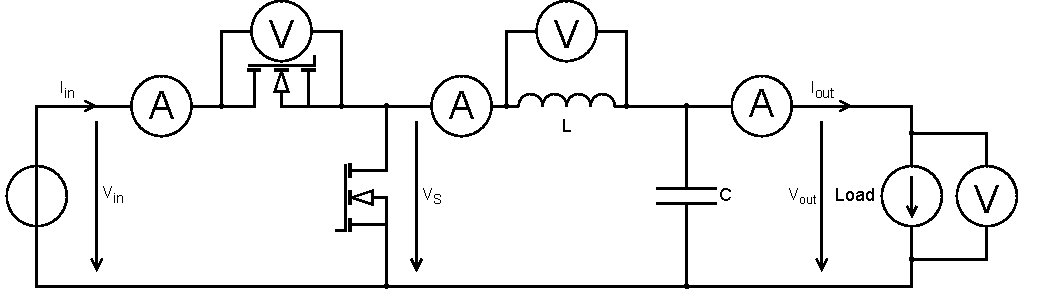
\includegraphics[width=1\linewidth]{Bilder/Kapitel4/BC_Measurement_Setup.pdf}
    \caption{Buck converter measurement setup}
    \label{fig:buck_converter_measurement_setup}
\end{figure}
The range of the switching frequency with which the buck converter can be controlled is limited by two factors. On the low end of the frequency spectrum, the ripple current amplitude increases exponentially. Because of this, the lowest analysed switching frequency is set to \SI{100}{\kilo\Hz}, avoiding saturation of the inductor. On the high end, the switching frequency is limited by the ability of the \ac{PWM} source. At over \SI{4}{\mega\Hz} the noise in the switching \ac{PWM} signal is too great to guarantee the reliant operation of the buck converter. Thus these two frequencies define the boundaries of the observed switching frequency range. A logarithmic sweep of six measurement frequencies is chosen to measure the behaviour of the buck converter: \SI{100}{\kilo\Hz}, \SI{300}{\kilo\Hz}, \SI{800}{\kilo\Hz}, \SI{1}{\mega\Hz}, \SI{2}{\mega\Hz} and \SI{4}{\mega\Hz}.
\begin{figure}[H]
    \begin{subfigure}[b]{0.50\textwidth}
        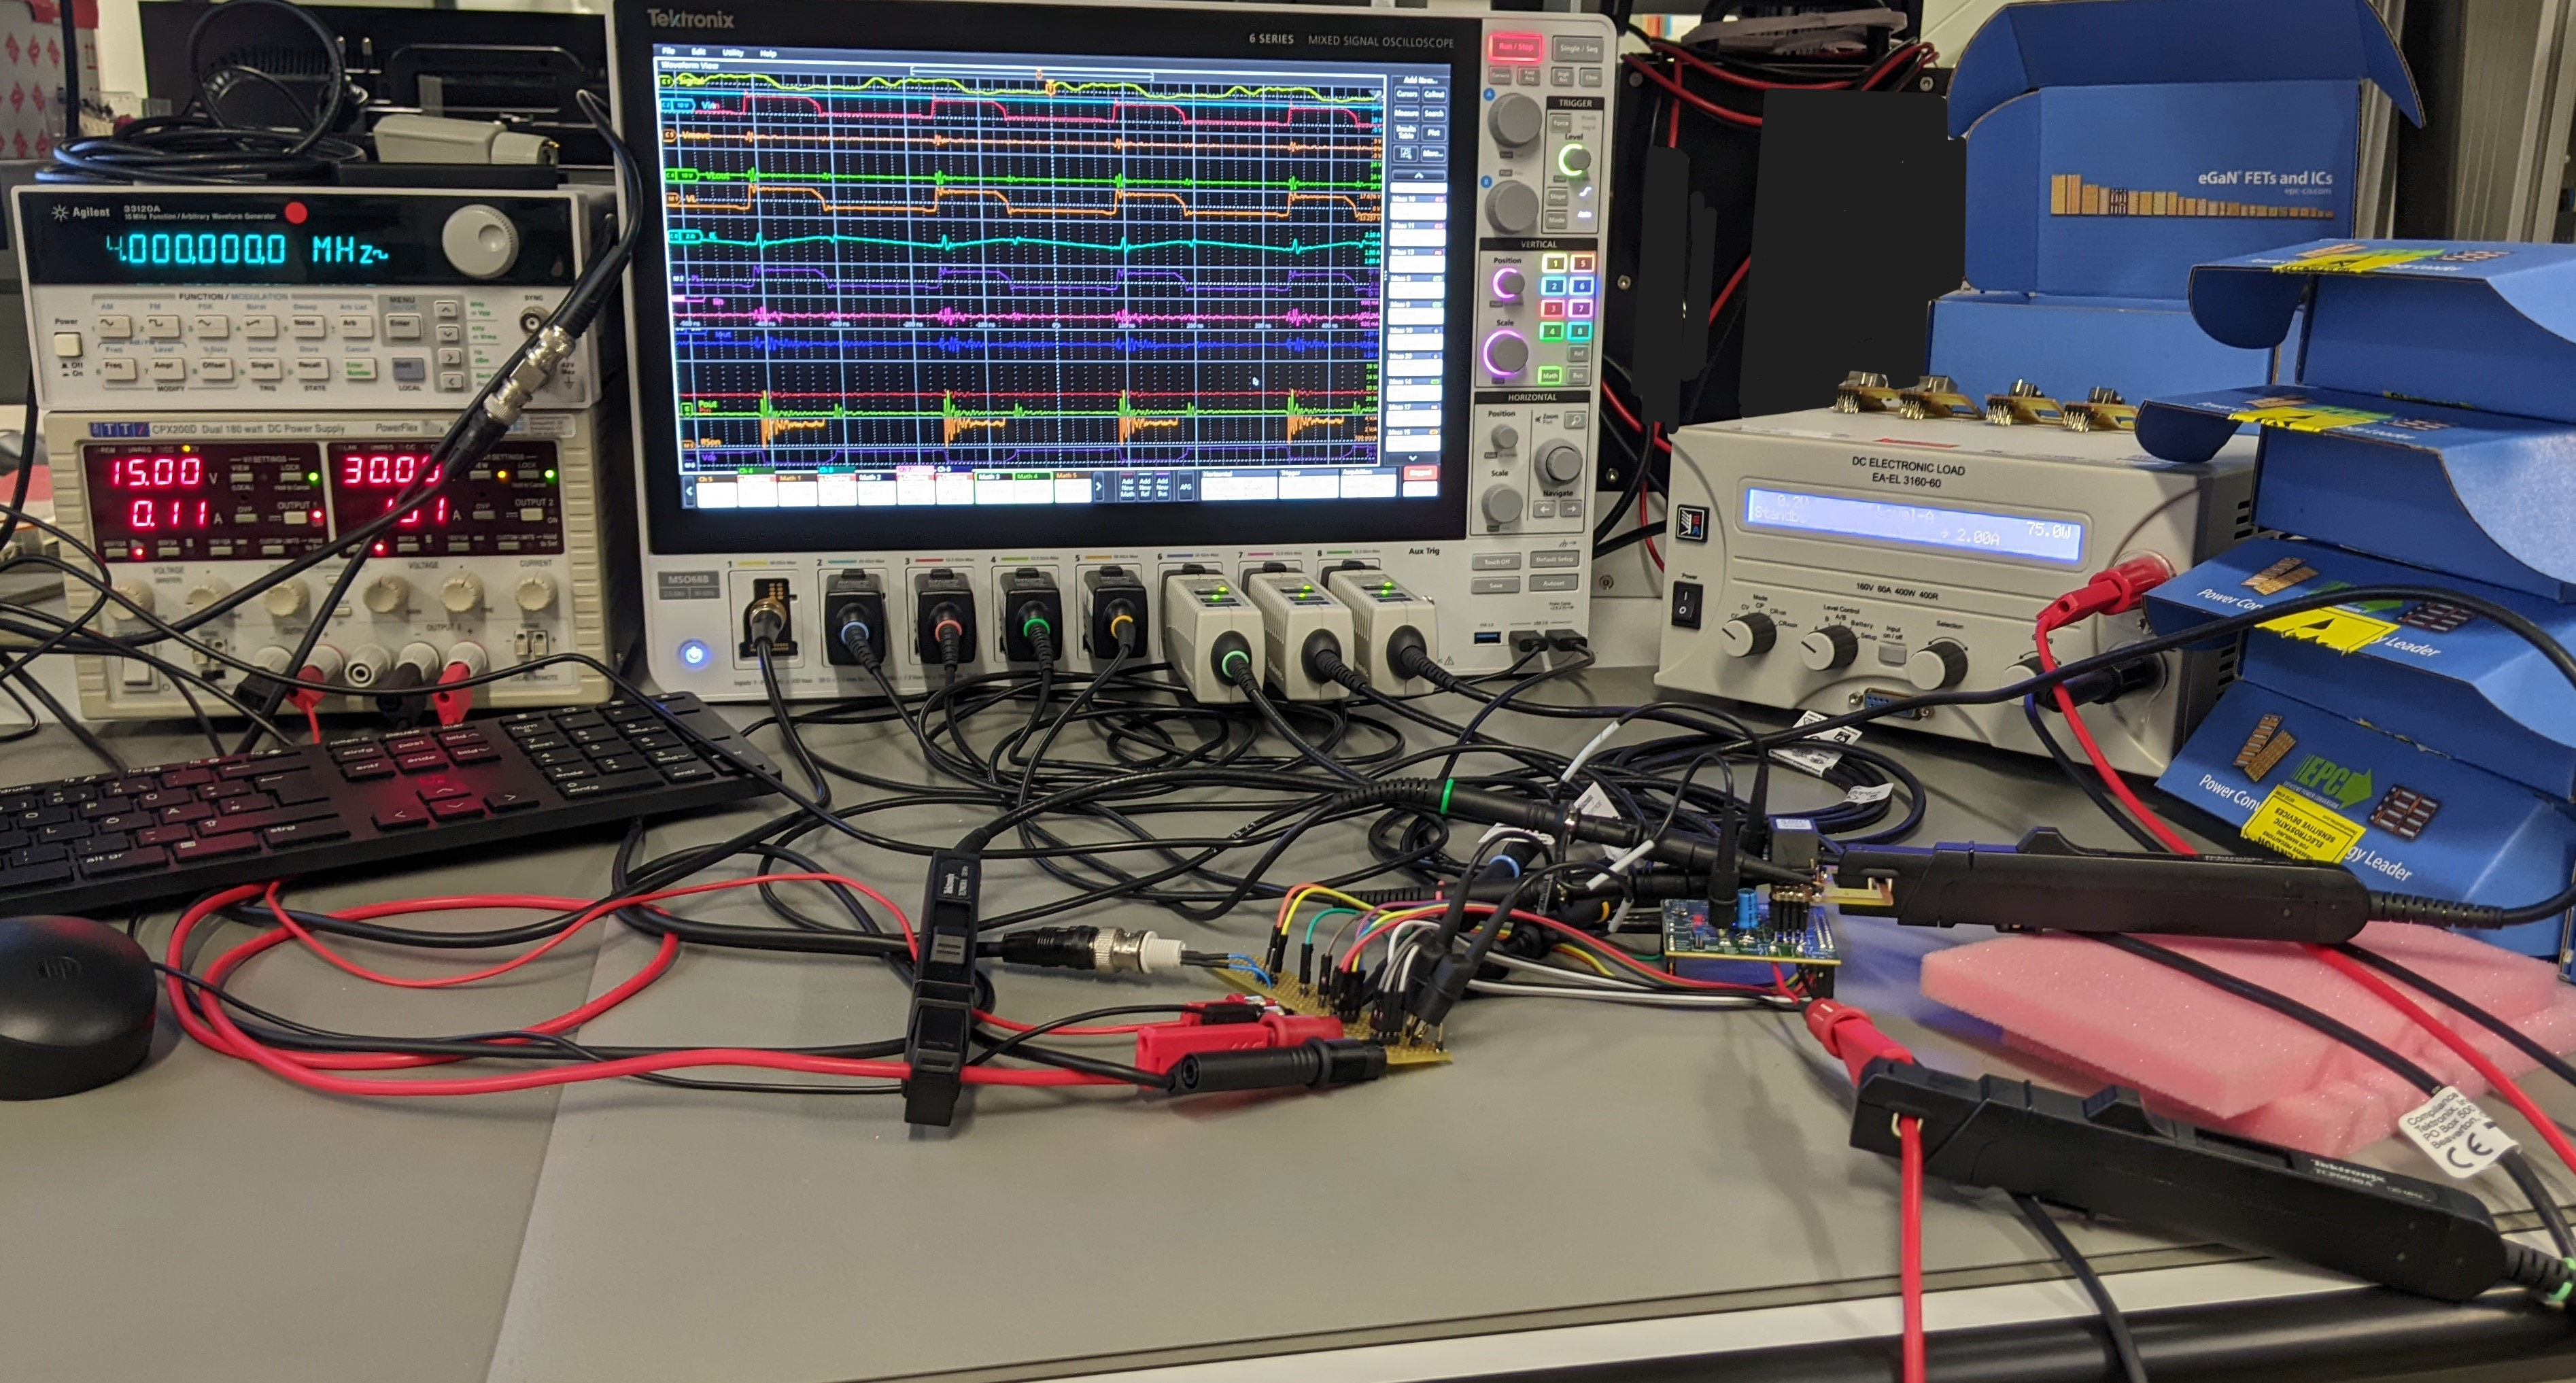
\includegraphics[width=\textwidth]{Bilder/Kapitel4/Measurement_Work_Station_cropped.jpg}
        \caption{Measurement equipment}
    \end{subfigure}
    \begin{subfigure}[b]{0.50\textwidth}
        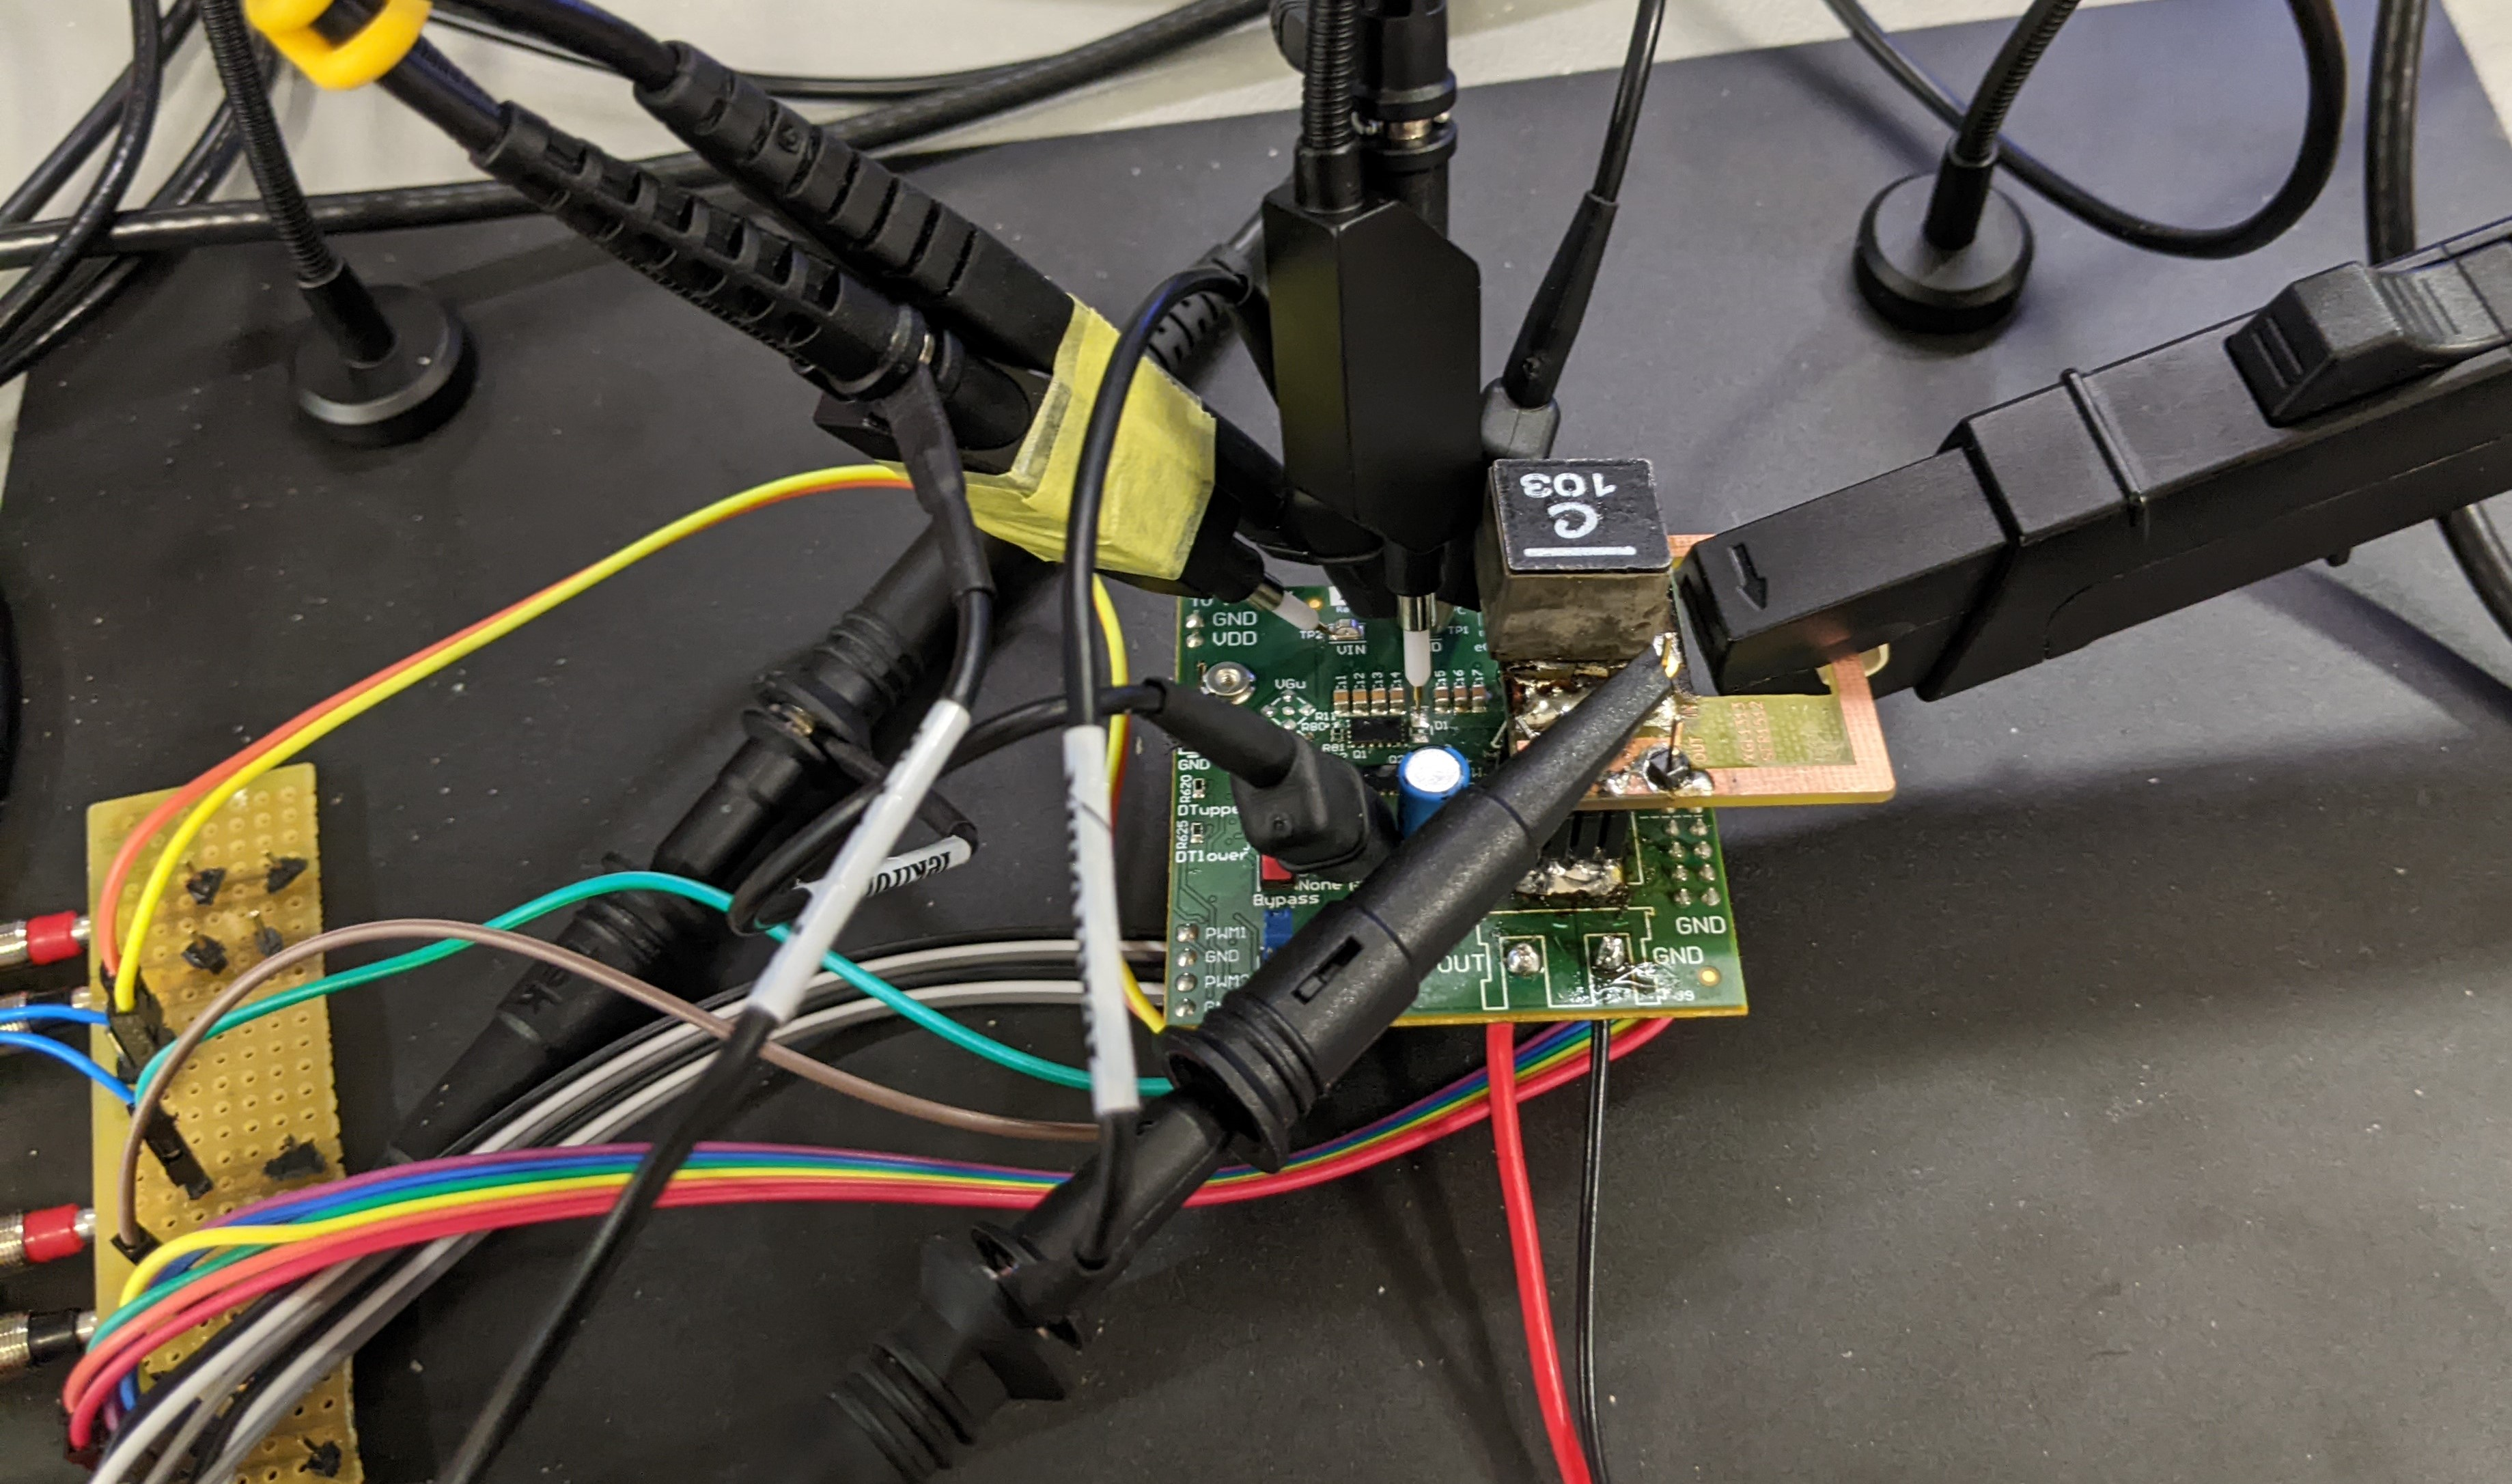
\includegraphics[width=\textwidth]{Bilder/Kapitel4/Measurement_Work_Station_close_cropped.jpg}
        \caption{Closeup of the buck converter}
    \end{subfigure}
    \caption{Physical measurement setup}
    \label{fig:hysteresis_comparison}							
\end{figure}

\section{Setup of the LTspice Buck Converter Measurement} \label{sec:setup_of_the_ltspice_buck_converter_measurement}
The physical model of the previous section is now recreated in LTspice, taking into account not just the inductor and \ac{GaNFET} losses, but also accounting for the losses in the capacitor and the \ac{PCB}.\\
For the capacitor, an \ac{ESR} is added based on a frequency-response measurement with the "Bode 100". From the measurement a resistance of approximately \SI{1}{$\Omega$} in the frequency range between \SI{100}{\kilo\Hz} and \SI{4}{\mega\Hz} is determined, setting this to be the value of the \ac{ESR}.\\
The resistance in the \ac{PCB} traces is determined for the section between the \ac{HS} \ac{GaNFET} and inductor, as well as the section between inductor and capacitor. Using the results of a four-point measurement, a \SI{6}{\milli$\Omega$} \ac{ESR} is added at the input of the inductor and a \SI{25}{\milli$\Omega$} \ac{ESR} is added at the output of the inductor.\\\\
The complete buck converter is then created based on figure \ref{fig:synch_buck_converter_2}, using the GaNFET models provided by EPC, inserting the validated inductor \ac{ECM} with saturation and accounting for the losses in the capacitor and \ac{PCB} traces.
\begin{figure}[H]
    \centering
    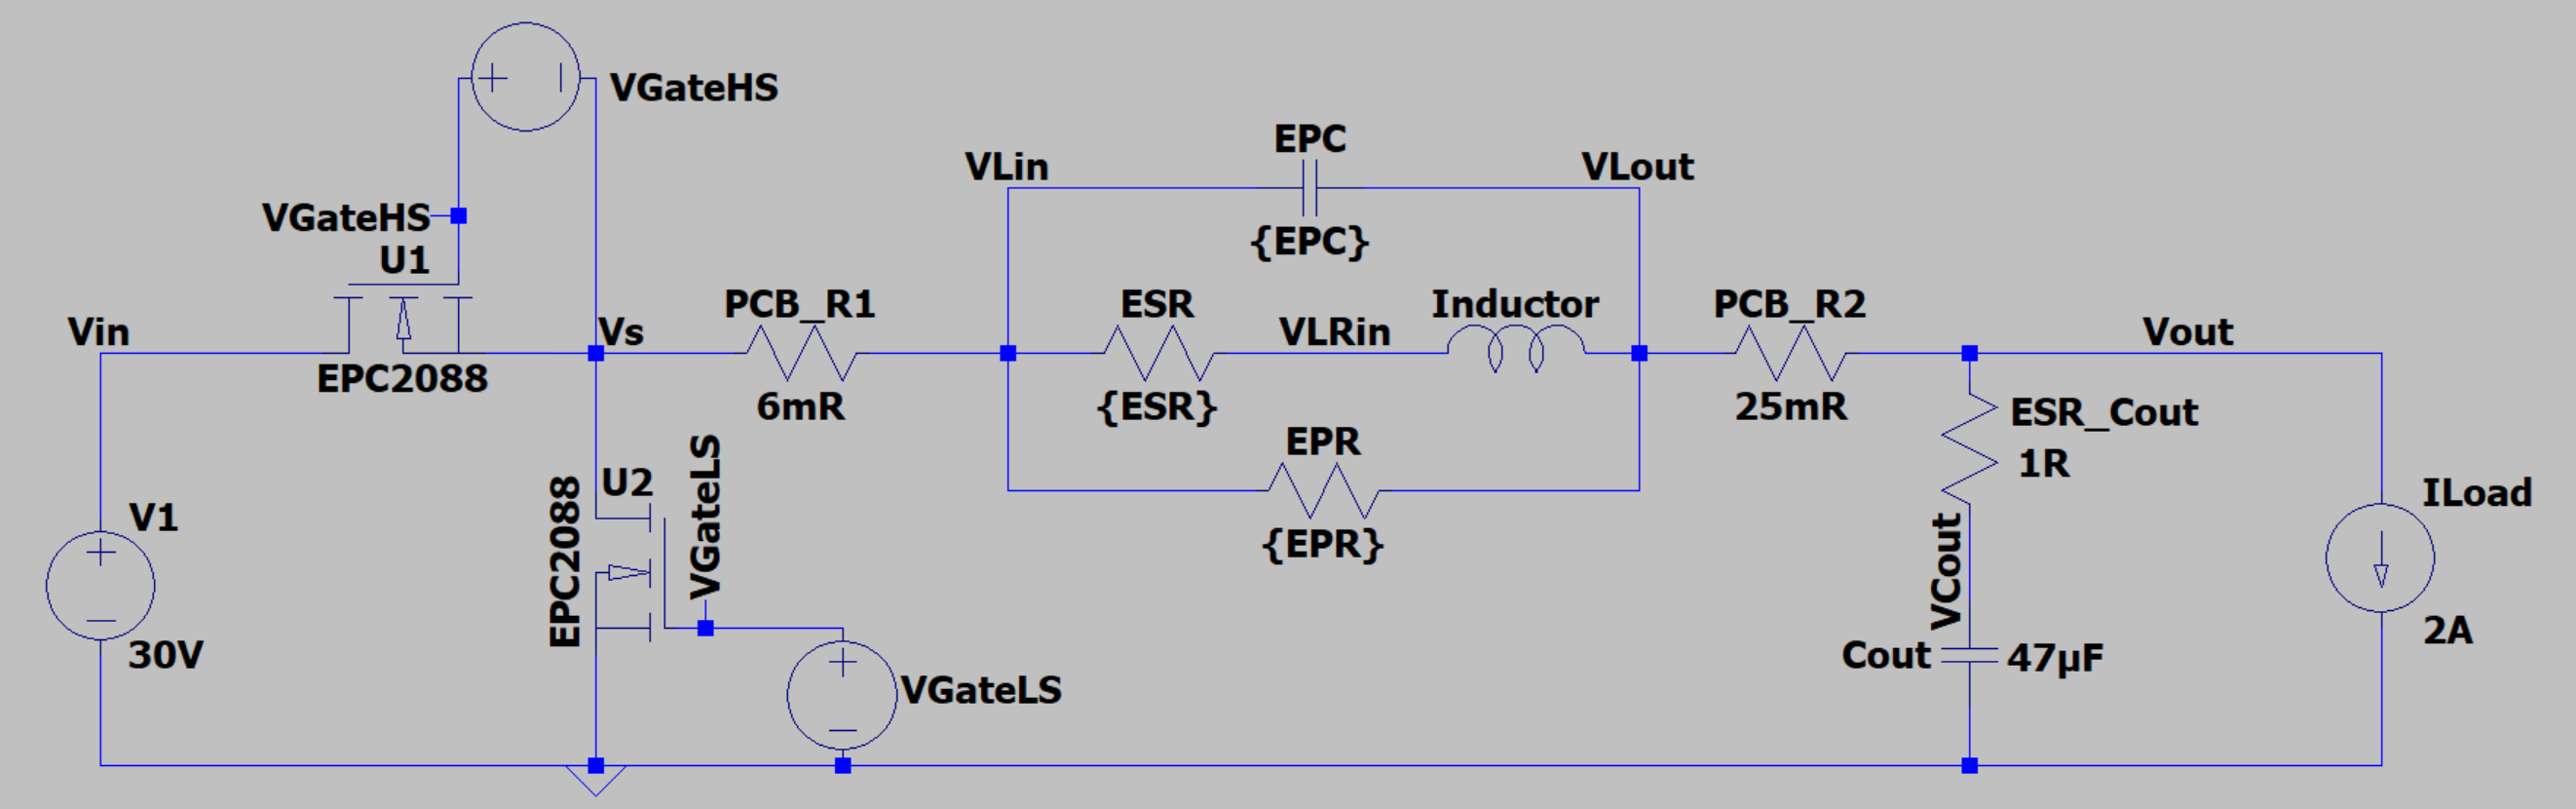
\includegraphics[width=1\linewidth]{Bilder//Kapitel4/BC_LTspice.png}
    \caption{Complete Synchronous Buck Converter in LTspice with the \textit{EPC2088}}
    \label{fig:BC_LTspice}
\end{figure}
Each \ac{GaNFET} is controlled by a voltage source connected between the \ac{GaNFET}'s source and gate, applying a \SI{6.3}{\V} rectangular signal in accordance with the switching frequency and dead time. 
The different equivalent circuit parameters for the individual inductors are stored in a table and stepped through in each simulation. For the saturation, a piecewise function is created containing all saturation functions, which are then selected based on the active inductor model. Enabling the switching between the different \acp{GaNFET} cannot be realised in the same way, as they are implemented as subnets, necessitating a separate buck converter model for each \ac{GaNFET}. The input voltage source is changed to output a constant \SI{30}{\V}.\\\\
Measuring the individual currents, voltages and powers is done via the \textit{.meas}-command, which outputs the average of the observed functions for each given switching frequency and buck converter to an external file. To calculate this average, LTspice simply adds up the values of its output graph, only taking into account the displayed part of the signal. Because of this, it is crucial that always a whole number of periods is displayed, to create an accurate measurement. The buck converter is therefore given a set amount of time to settle after which ten periods are displayed and used for the measurements. 






% The results of section \ref{sec:complete_simulation_of_the_buck_converter} show how the behaviour of a given synchronous buck converter can be approximated by LTspice. Incorporating the \ac{ECM} of the used inductor and a fitting model for the switching element, yield loss simulations that approximate the true behaviour and deliver insights about the efficiency characteristics of the observed synchronous buck converter. These simulations however have non-negligible shortcomings. As the sole \ac{ECM} is not able to truly represent the core losses, the losses of the inductor are only a rough approximation of the actually occurring losses. Due to hysteresis and the effect of \ac{DC} bias not being able to be represented by a simple \ac{ECM}, another method is necessary to reduce the error of the simulation. Yet, as shown in section \ref{sec:hysteresis_behaviour_of_the_inductor}, the LTspice inbuilt hysteresis solver is not capable of providing a fitting solution.\\
% Apart from the inductor, section \ref{sec:simulating_the_buck_converter} shows that the provided \ac{GaNFET} models also do not behave like their physical counterparts. While their switching losses are well-modelled, the low-frequency losses measured in the buck converter are not represented by the model.\\
% Taking these inaccuracies into account, the LTspice model is still able to provide an estimate of the ideal switching frequency for a given synchronous buck converter. Running the simulation for smaller frequency increments shows how the simulation gives bounds in which the ideal switching frequency lays. 
% \begin{figure}[H]
%     \centering
%     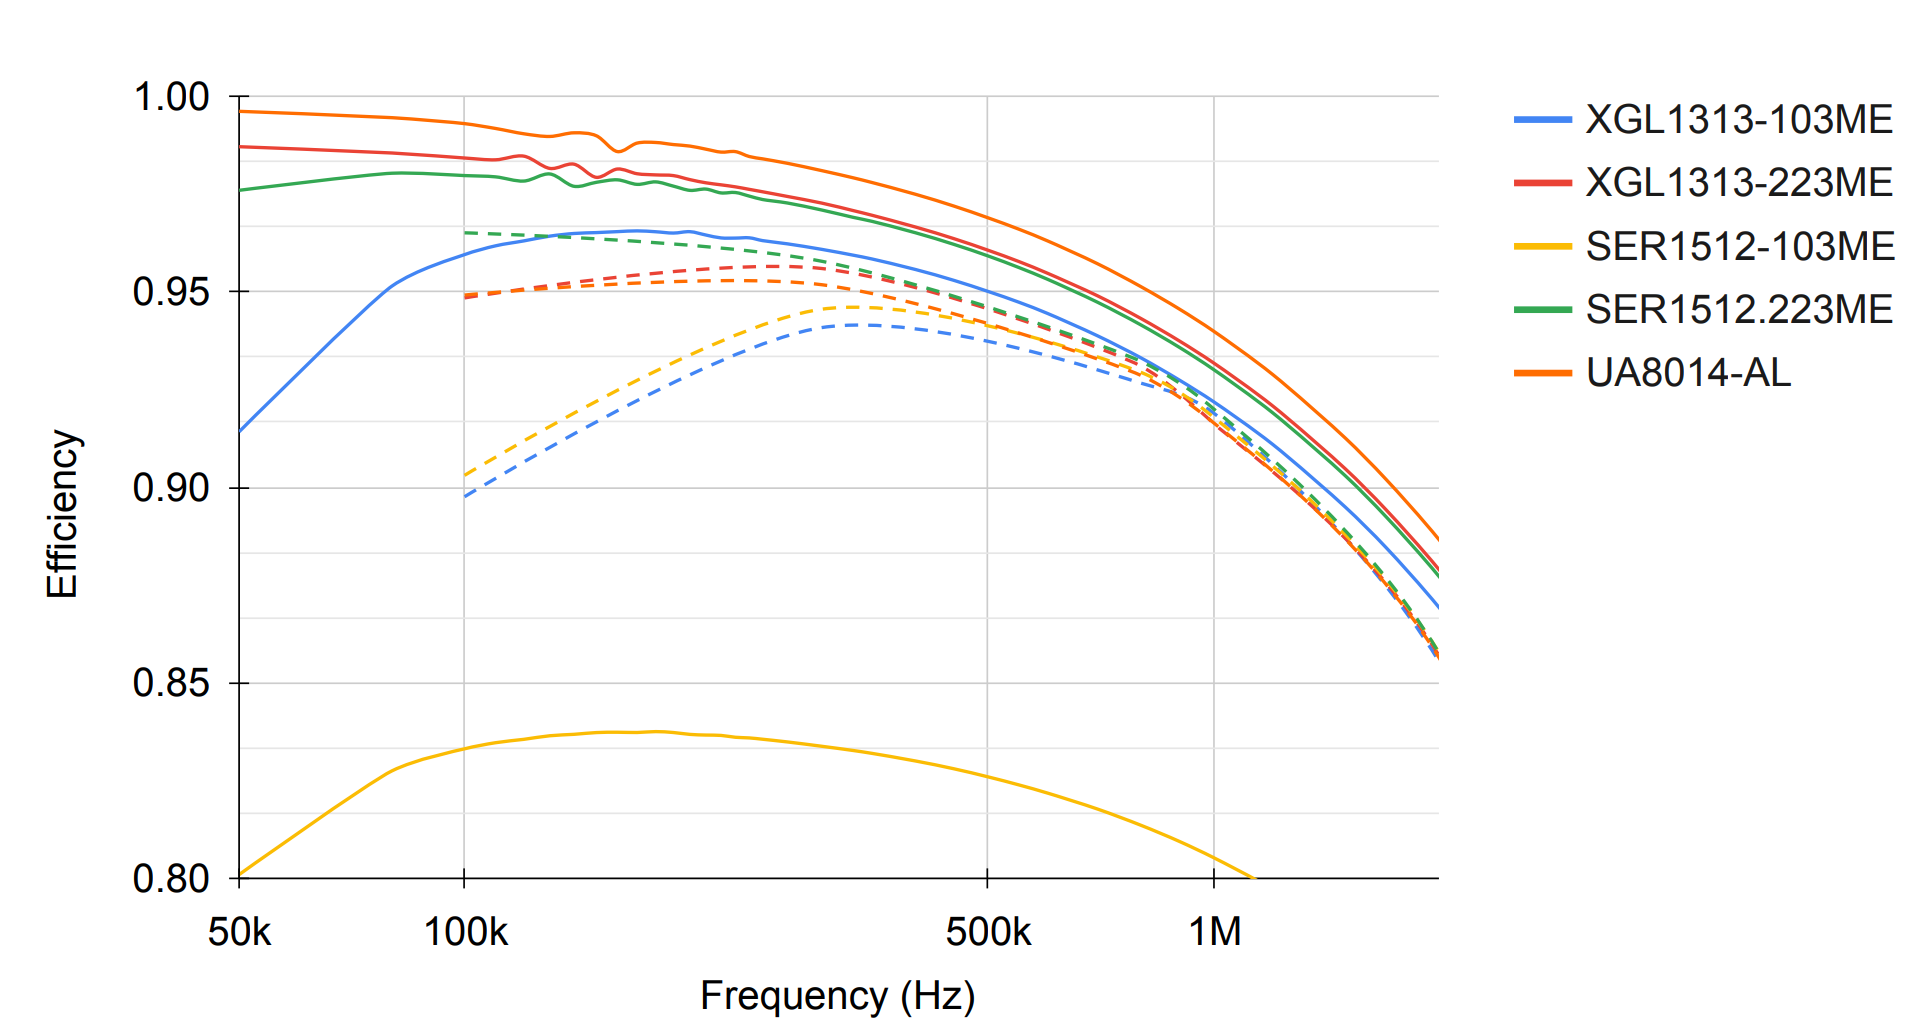
\includegraphics[width=1\linewidth]{Bilder/Kapitel4/Efficiency_Simulation_Comparison.png}
%     \caption{Comparison of the simulated and measured efficiency of the different buck converters all using the \textit{EPC2088} \ac{GaNFET} \\striped lines indicate measured values, while continuous lines are simulated}
%     \label{fig:efficiency_simuilation_comparison}
% \end{figure}
% Demonstrated by the buck converter of the \textit{XGL1313-103ME} inductor and \textit{EPC2088} \ac{GaNFET}, the simulation defines a range between \SI{80}{kHz} and \SI{500}{kHz}, where the efficiency is at a maximum. This coincides with the measurement, which predicts an ideal switching frequency of \SI{300}{kHz}. Hence, this estimation can then be used to determine the true ideal switching frequency through real-world measurements. 


























% \chapter{Results and Discussion}
% \label{sec:cha5}
% The created model is simulated for the same \acp{GaNFET} and inductors that are used in the physical buck converter and evaluated compared to the results of section \ref{sec:measuring_the_buck_converter}.



% Having laid the foundation for an LTspice inductor model and explained the limits of the inbuilt hysteresis model, the simulated inductor is now compared to a physical inductor. First, a setup to measure the voltages and currents of a synchronous buck converter is presented in section \ref{sec:buck_converter_measurement}. Its resulting measurements are assessed for expected behaviour, removing measurement errors. The setup is then used in section \ref{sec:validation_of_the_inductor_saturation_model} to validate the saturation model created in section \ref{sec:saturation_behaviour_of_the_inductor} by comparing the ripple current behaviour for different currents through the inductor. Combining the results in section \ref{sec:complete_simulation_of_the_buck_converter}, a complete synchronous buck converter is recreated in LTspice, by incorporating the provided \ac{GaNFET} models. The simulated losses are then compared to the measured losses and an approach to estimate the ideal switching frequency is proposed in section \ref{sec:evaluation}. 

% \section{Buck Converter Measurement}\label{sec:buck_converter_measurement}
% To compare the simulation to real-world measurements, multiple buck converters are built and measured. First, the parts, equipment and settings used for the physical measurements are discussed. After that, the results of the measurements are presented and evaluated based on the theory introduced in chapter \ref{sec:fundamentals}.

% \subsection{Simulating the Buck Converter}\label{sec:simulating_the_buck_converter}
% To compare the results of the simulation with those of the measurement, the different combinations of inductors and \acp{GaNFET} are simulated at the same switching frequencies used in the measurements. The buck converter with the inductor \textit{XGL1313-103ME} is again used to present the different efficiency behaviours of the \acp{GaNFET}. In the following figure, the simulated efficiencies are directly compared to the results of the measurements of section \ref{sec:measuring_the_buck_converter}. 
% \begin{figure}[H]
%     \begin{subfigure}[b]{0.50\textwidth}
%         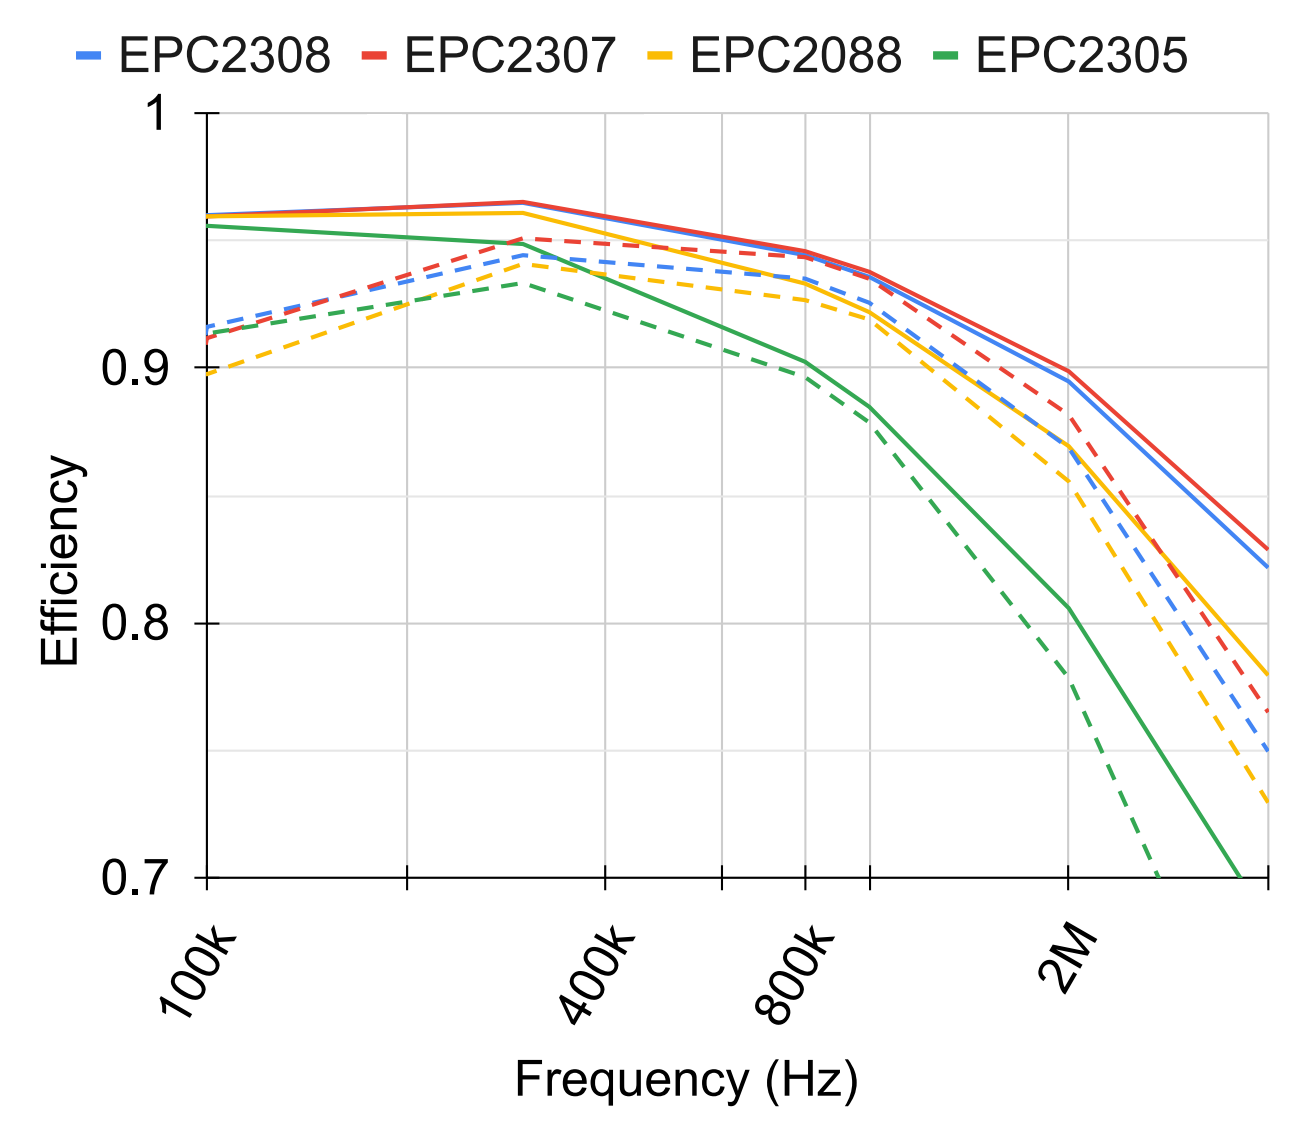
\includegraphics[width=\textwidth]{Bilder/Kapitel4/XGL103 Efficiency Simulated and measured.png}
%     \end{subfigure}
%     \begin{subfigure}[b]{0.50\textwidth}
%         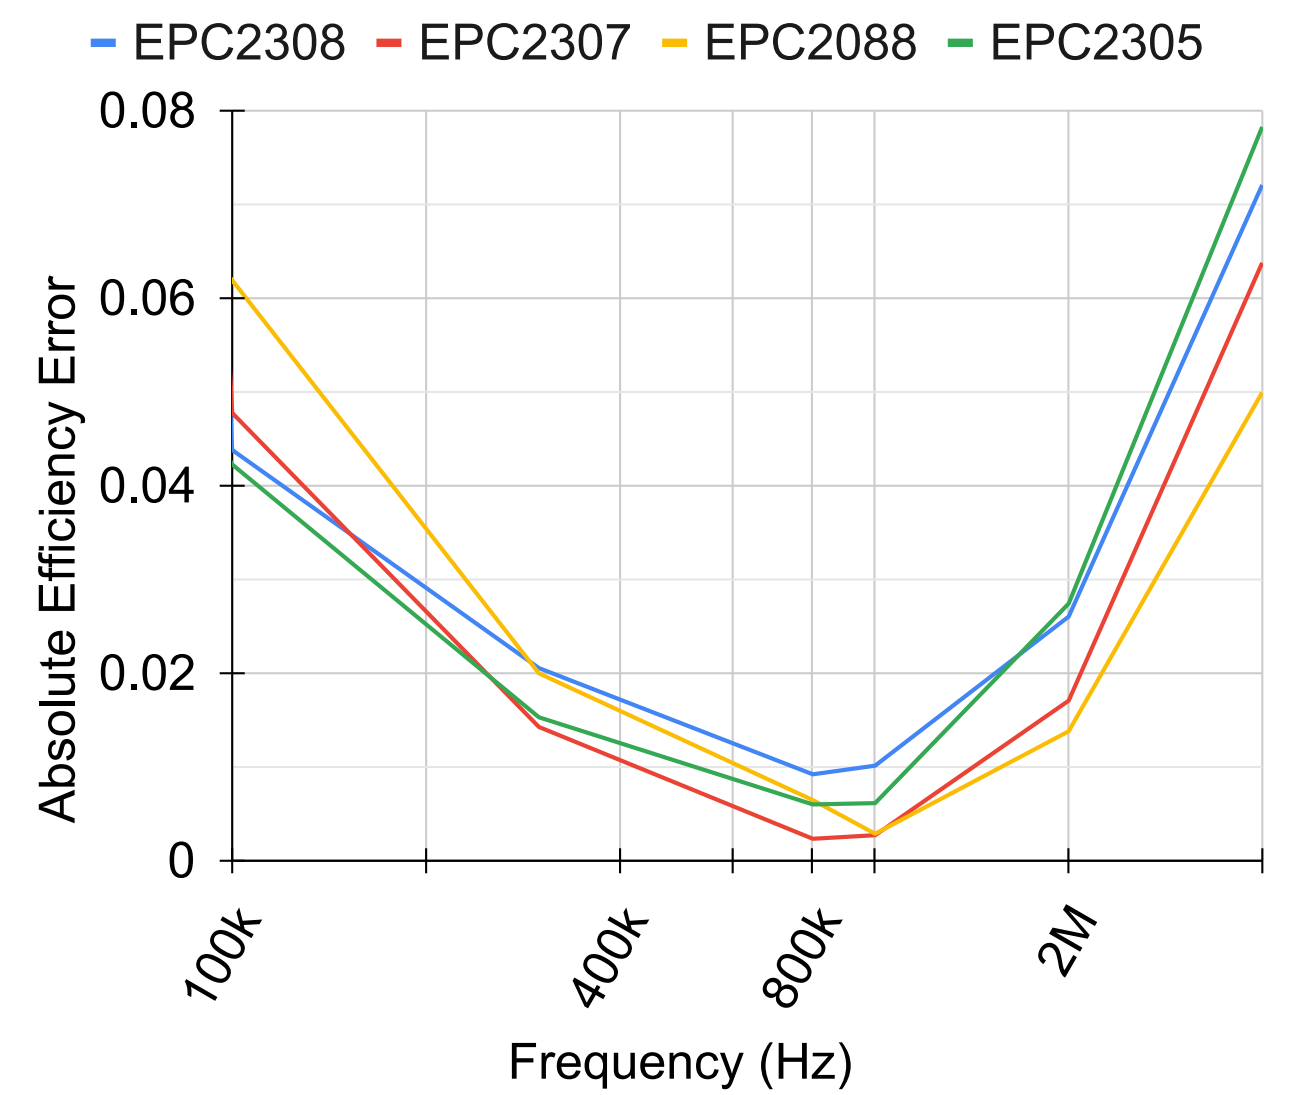
\includegraphics[width=\textwidth]{Bilder/Kapitel4/XGL103 Efficiency Simulated and measured error.png}
%     \end{subfigure}
%     \caption{Comparison of the simulated and measured buck converter's efficiencies for the \textit{XGL1313-103ME} inductor\\striped lines indicate measured values, while continuous lines are simulated}
%     \label{fig:comparison_efficiencies_sim_and_meas}							
% \end{figure}
% A noticeable error of around 5\% for all Types of \acp{GaNFET} appears at the low end of the frequency range. With increasing frequency the simulation first approaches the measured efficiency, reaching a minimal error of less than 1\% at a switching frequency of \SI{1}{\mega\Hz}, after which the error again increases. Overall the efficiency in the simulation is higher, than the measured efficiency, hinting at physical losses that are not represented in the simulation. Still, the approximate shape of the simulated efficiency curve follows that of the measured efficiency curve.\\
% Taking a closer look at the loss distribution of an individual buck converter shown in figure \ref{fig:xgl103_epc2088_loss_comparison}, gives an insight into the missing loss sources. To keep the example used in section \ref{sec:measuring_the_buck_converter}, the buck converter using the \textit{XGL1313-103ME} inductor and the \ac{GaNFET} \textit{EPC2088} is examined. Firstly, the simulation shows a linear rise in the \ac{GaNFET} losses in respect to the switching frequency, showing that the switching losses are represented by the simulation. At low switching frequencies, the model however deviates from the expected behaviour, as the losses in the \ac{GaNFET} are now attributed mainly to effects, other than the switching losses.\\
% Similarly, the behaviour of the simulated inductor also strays from the measured behaviour. At low switching frequencies, the simulated inductor losses start out high and begin to decrease as the frequency increases. While this reduction continues on in the measured inductor, it halts for the simulated inductor. The simulated inductor thereby undershoots the losses at low frequencies and overshoots the measured losses at high frequencies.
% \begin{figure}[H]
%     \centering
%     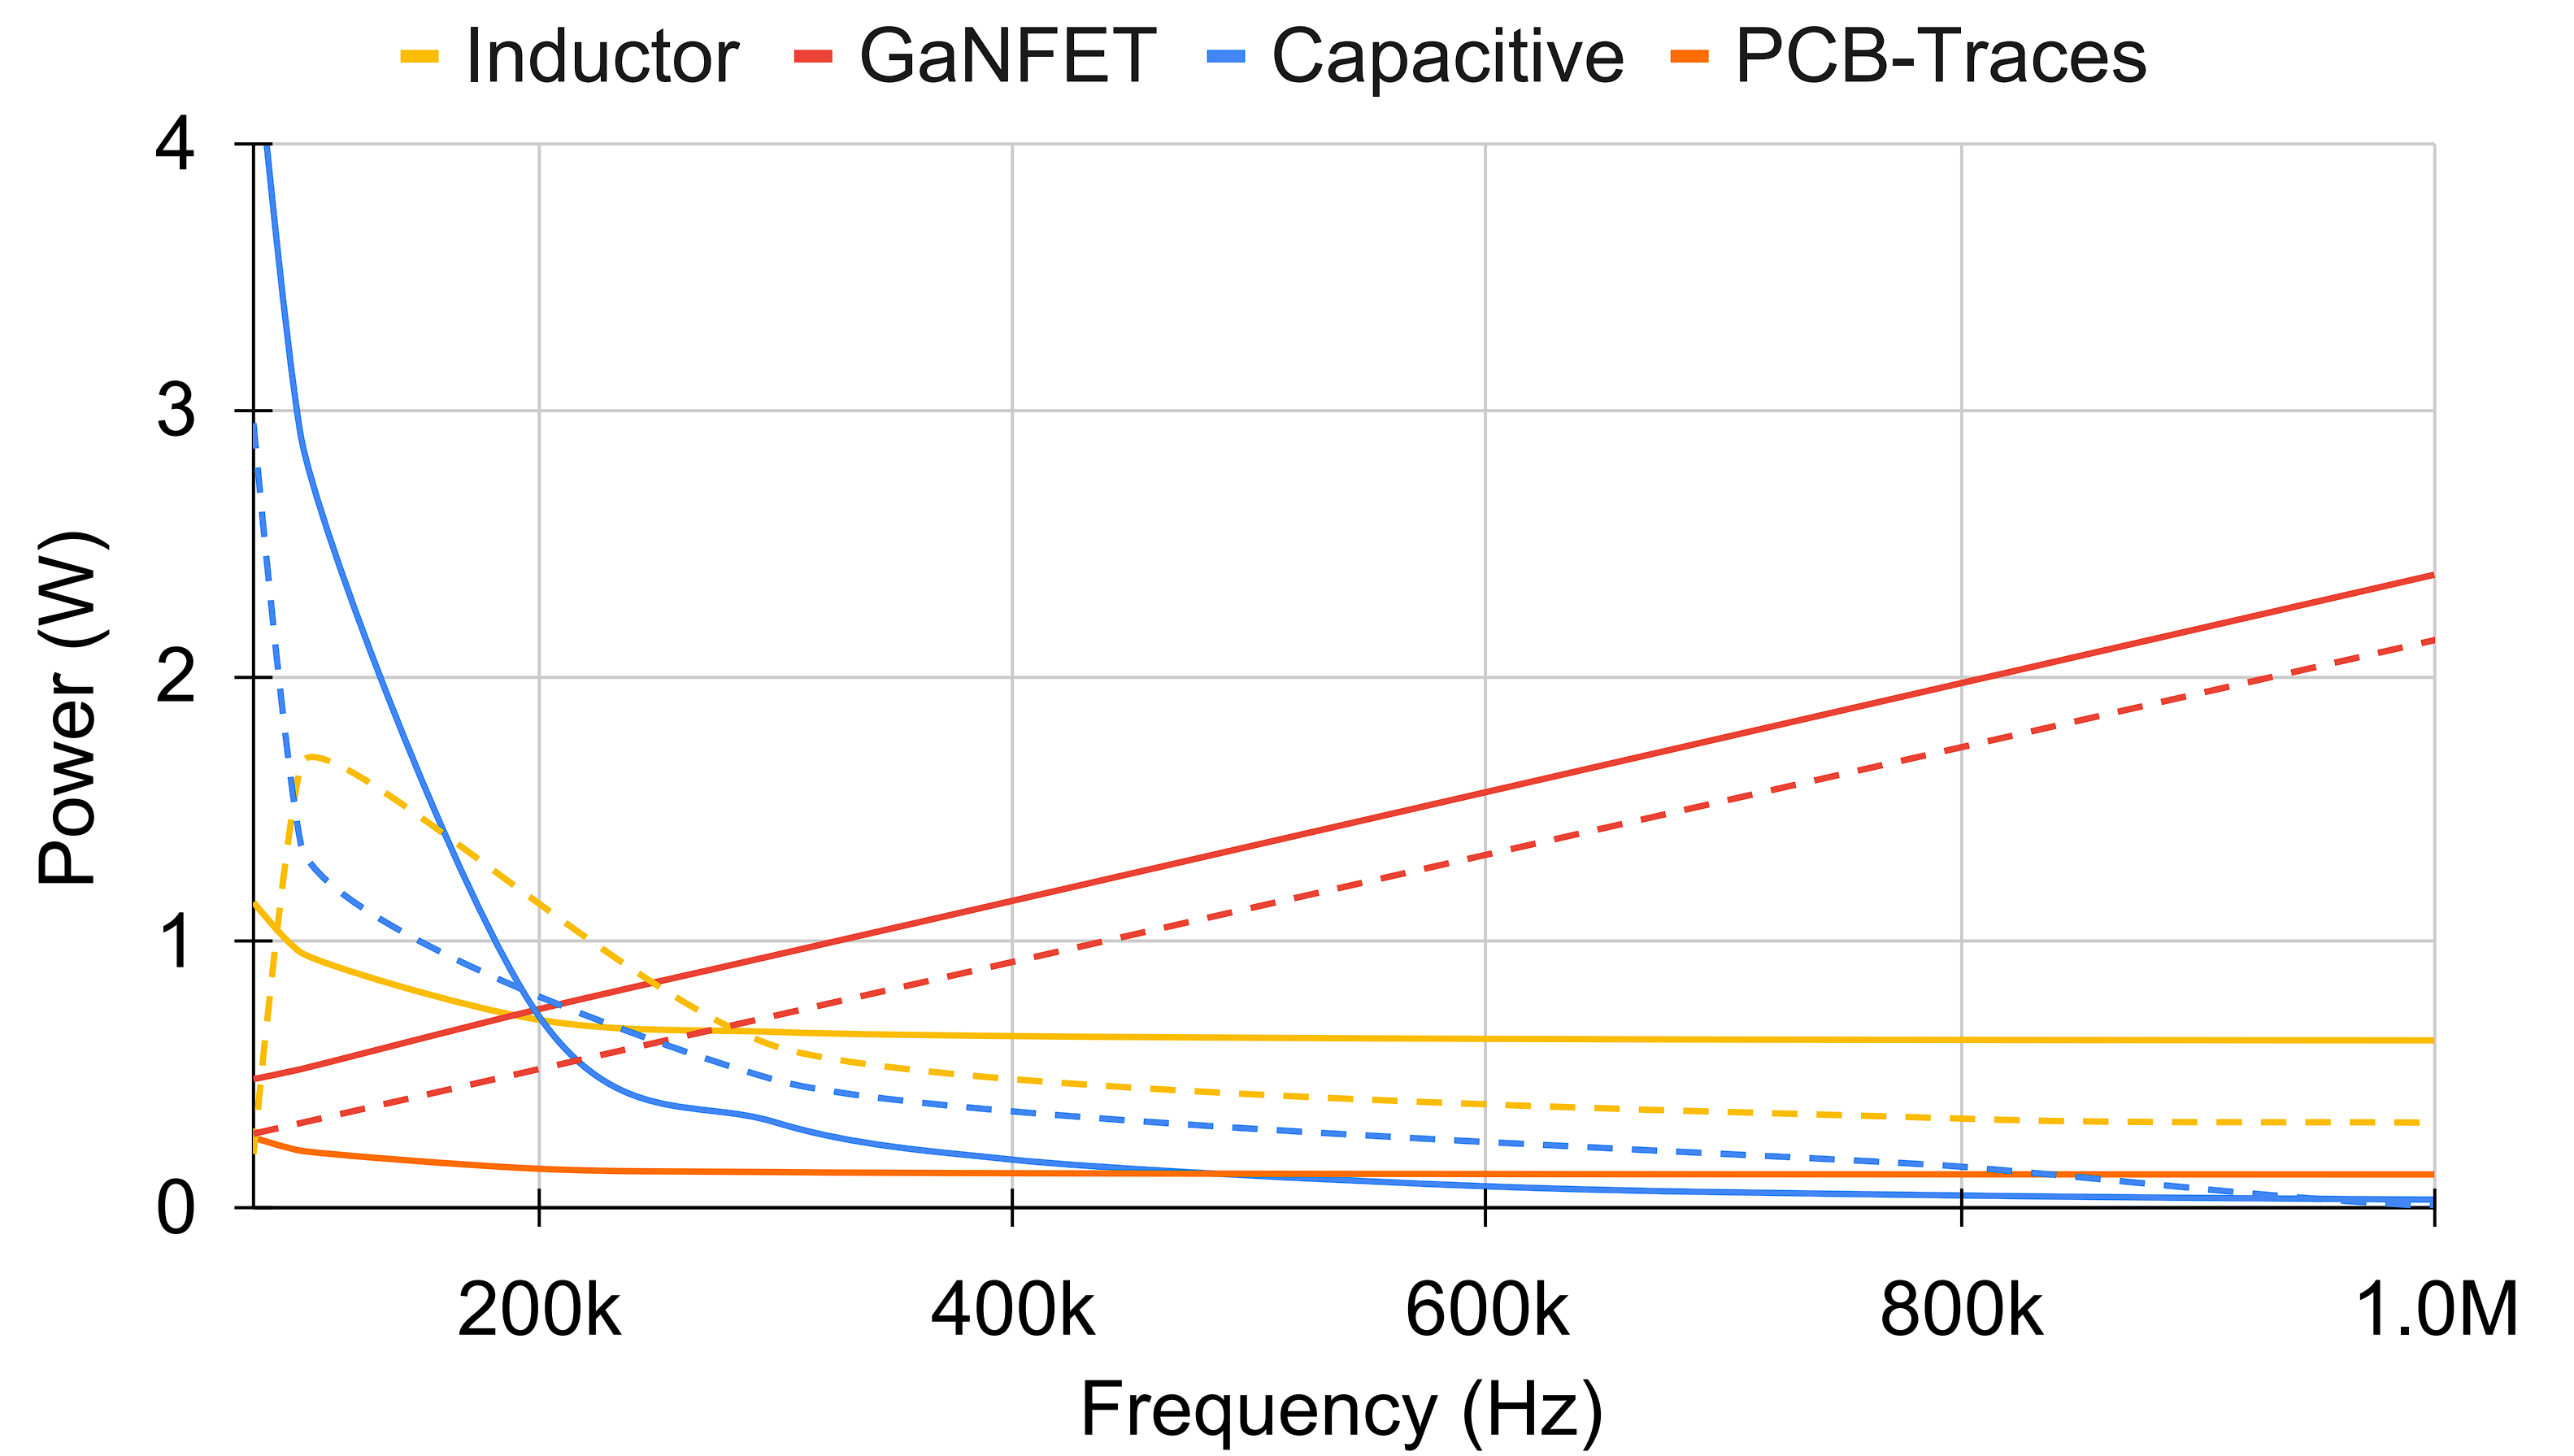
\includegraphics[width=0.75\linewidth]{Bilder/Kapitel4/XGL103_EPC2088_Simulation_Loss_Comparison.png}
%     \caption{Comparison of the inductor and switching losses for the buck converter consisting of the \textit{XGL1313-103ME} inductor and \textit{EPC2088} \acp{GaNFET}}
%     \label{fig:xgl103_epc2088_loss_comparison}
% \end{figure}
% Transferring the individual loss behaviour of the simulation back to figure \ref{fig:comparison_efficiencies_sim_and_meas}, shows that this difference in behaviour is not only observed for this specific buck converter but across all four different buck converters with the \textit{XGL1313-103ME} inductor. In fact, this discrepancy between the measured and simulated behaviour holds true for all observed buck converters.

%--> Comparison of the measured and simulated values --> At what frequency is the buck converter optimal? (does this approach the same point, as measured
%--> What are the differences, why is the efficiency so much higher, than in real life?
%--> How big is the error, and is it usable?
 
% \section{Evaluation}\label{sec:evaluation}
% The results of section \ref{sec:complete_simulation_of_the_buck_converter} show how the behaviour of a given synchronous buck converter can be approximated by LTspice. Incorporating the \ac{ECM} of the used inductor and a fitting model for the switching element, yield loss simulations that approximate the true behaviour and deliver insights about the efficiency characteristics of the observed synchronous buck converter. These simulations however have non-negligible shortcomings. As the sole \ac{ECM} is not able to truly represent the core losses, the losses of the inductor are only a rough approximation of the actually occurring losses. Due to hysteresis and the effect of \ac{DC} bias not being able to be represented by a simple \ac{ECM}, another method is necessary to reduce the error of the simulation. Yet, as shown in section \ref{sec:hysteresis_behaviour_of_the_inductor}, the LTspice inbuilt hysteresis solver is not capable of providing a fitting solution.\\
% Apart from the inductor, section \ref{sec:simulating_the_buck_converter} shows that the provided \ac{GaNFET} models also do not behave like their physical counterparts. While their switching losses are well-modelled, the low-frequency losses measured in the buck converter are not represented by the model.\\
% Taking these inaccuracies into account, the LTspice model is still able to provide an estimate of the ideal switching frequency for a given synchronous buck converter. Running the simulation for smaller frequency increments shows how the simulation gives bounds in which the ideal switching frequency lays. 
% \begin{figure}[H]
%     \centering
%     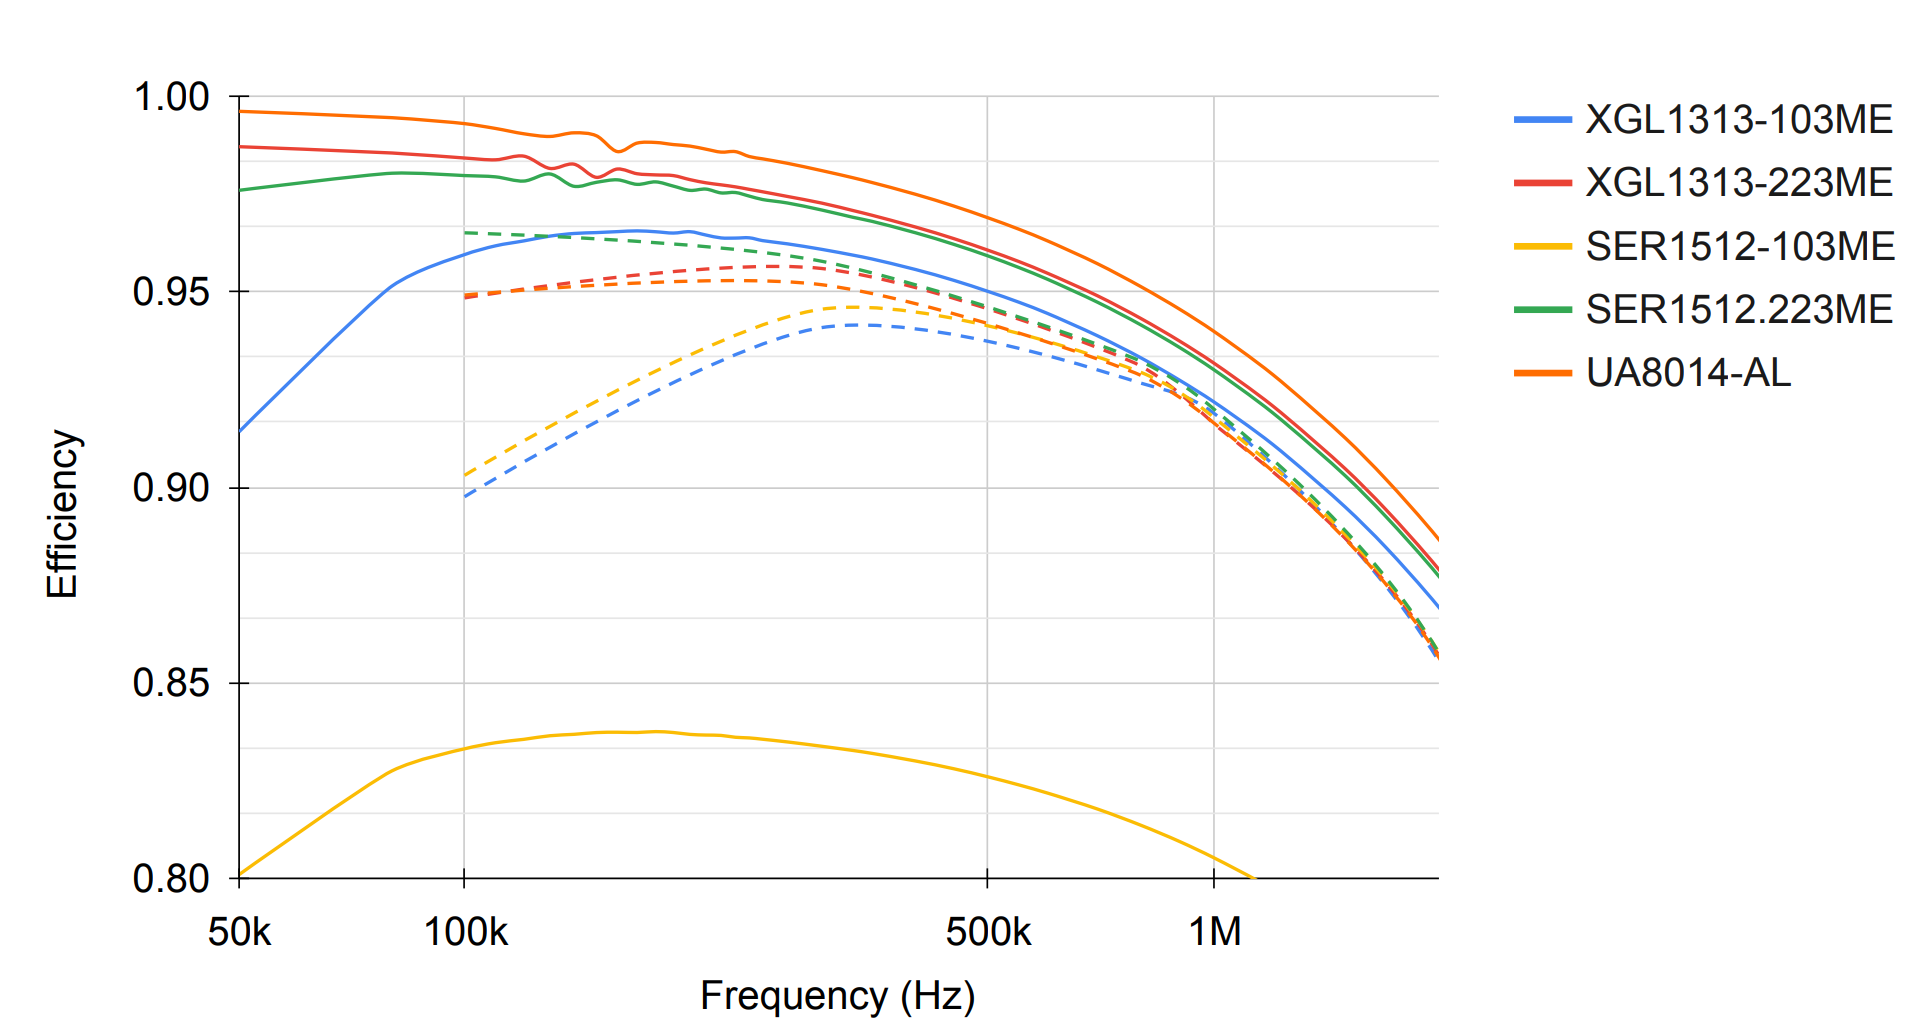
\includegraphics[width=1\linewidth]{Bilder/Kapitel4/Efficiency_Simulation_Comparison.png}
%     \caption{Comparison of the simulated and measured efficiency of the different buck converters all using the \textit{EPC2088} \ac{GaNFET} \\striped lines indicate measured values, while continuous lines are simulated}
%     \label{fig:efficiency_simuilation_comparison}
% \end{figure}
% Demonstrated by the buck converter of the \textit{XGL1313-103ME} inductor and \textit{EPC2088} \ac{GaNFET}, the simulation defines a range between \SI{80}{kHz} and \SI{500}{kHz}, where the efficiency is at a maximum. This coincides with the measurement, which predicts an ideal switching frequency of \SI{300}{kHz}. Hence, this estimation can then be used to determine the true ideal switching frequency through real-world measurements. 



%--> Is this method feasible, does it help? Where are the limitations?
%\todo[inline]{Validate the inductor ECM}
%\todo[inline]{Validate the saturation model}
%\todo[inline]{Explain the Buck Converter Measurement Setup, in the lab and in LTspice}
%\todo[inline]{Compare the losses of both measurments}

%\todo[inline]{Evaluate the accuracy}
%\todo[inline]{Explain the short commings of the work --> Show the error}
%\todo[inline]{Goal --> Repeatability has to be reservered (all necessary data to repeat the experiments needs to be mentioned)}